\documentclass{beamer}
\usetheme{Madrid}
\usepackage{minted}
% sudo tlmgr install minted
\usepackage[utf8]{inputenc}
\usepackage[T2A]{fontenc}
\usepackage[russian,english]{babel}

% Footline: show current section (left) and frame numbers (right)
\setbeamertemplate{footline}{%
  \leavevmode%
  \hbox{%
    \begin{beamercolorbox}[wd=.78\paperwidth,ht=2.5ex,dp=1ex,left]{author in head/foot}%
      \hspace*{1em}\usebeamerfont{footline}\insertsectionhead%
    \end{beamercolorbox}%
    \begin{beamercolorbox}[wd=.22\paperwidth,ht=2.5ex,dp=1ex,right]{date in head/foot}%
      \usebeamerfont{footline}\insertframenumber{} / \inserttotalframenumber\hspace*{1em}%
    \end{beamercolorbox}%
  }%
}

\newcommand{\parpause}[1]{\only<+->{#1\par}}
\newenvironment{definitionbox}[1][Определение]{%
  \begin{exampleblock}{#1}
}{%
  \end{exampleblock}
}

\AtBeginSection[]
{
  \begin{frame}
    \frametitle{Содержание}
    \tableofcontents[currentsection]
  \end{frame}
}

\title{Семинар 6. Модели согласованности, сериализуемость и транзакционность}
\subtitle{Распределенные вычисления}
\author{Георгий Семенов}
\institute{Институт прикладных компьютерных наук \\ Университет ИТМО}
\date{весна 2026}

\begin{document}

\frame{\titlepage}

\begin{frame}
\frametitle{Организационные моменты}

\begin{itemize}
  \item (Напоминание) Второе домашнее задание – жесткий дедлайн в 23:59 02.04.2026
  \item Исправления по первому домашнему заданию
    \begin{itemize}
    \item $\geq 0.75$ – исправления не принимаются ("4" за задание есть)
    \item Просьба: не исправляйте! Делайте следующее задание :)
    \end{itemize}
\end{itemize}

\end{frame}

\section{Модели согласованности}

\begin{frame}
\frametitle{Понятие согласованности}

\begin{definitionbox}[Модель согласованности]
Модель системы, которая определяет, какие значения при чтении могут быть возвращены после записей.
\end{definitionbox}

\begin{itemize}
    \item На практике выражается как:
    \begin{itemize}
        \item Контракты и гарантии API к хранилищу данных
        \item Транзакционные уровни изоляции в СУБД
        \item Гарантии доставки сообщений в системах обмена сообщениями
    \end{itemize}

    \item Возникает и в других разделах computer science:
    \begin{itemize}
        \item Модели памяти в языках программирования (Java Memory Model, C++11)
    \end{itemize}

    \item Выделяют более {\itshape сильные} и более {\itshape слабые} модели согласованности
    \begin{itemize}
        \item Чем слабее модель, тем проще масштабироваться и выше доступность
        \item Чем сильнее модель, тем меньше аномалий, но выше задержка
    \end{itemize}
\end{itemize}

\end{frame}

\begin{frame}
\frametitle{Consistency vs. Integrity}

\begin{columns}
\column{0.5\textwidth}
\textbf{Consistency (согласованность)}
\begin{itemize}
  \item Какие допустимые состояния системы видны нам после изменения
  \item Должны ли мы видеть обновление? С какой допустимой задержкой? В каком порядке?
  \item Пример: read-your-writes (session consistency)
\end{itemize}

\column{0.5\textwidth}
\textbf{Integrity (целостность)}
\begin{itemize}
  \item Какие состояния запрещены инвариантами
  \item Пример: \texttt{balance >= 0}, уникальность email
\end{itemize}
\end{columns}

\vspace{0.3cm}
\begin{alertblock}{Важно}
По-русски «согласованность» и «целостность» иногда путают, но это разные вещи.
\end{alertblock}

\end{frame}

\begin{frame}
\frametitle{Некоторые важные модели по M. Perrin}

\begin{columns}
    \column{0.5\textwidth}
        \begin{center}
            \vspace*{-1cm}
            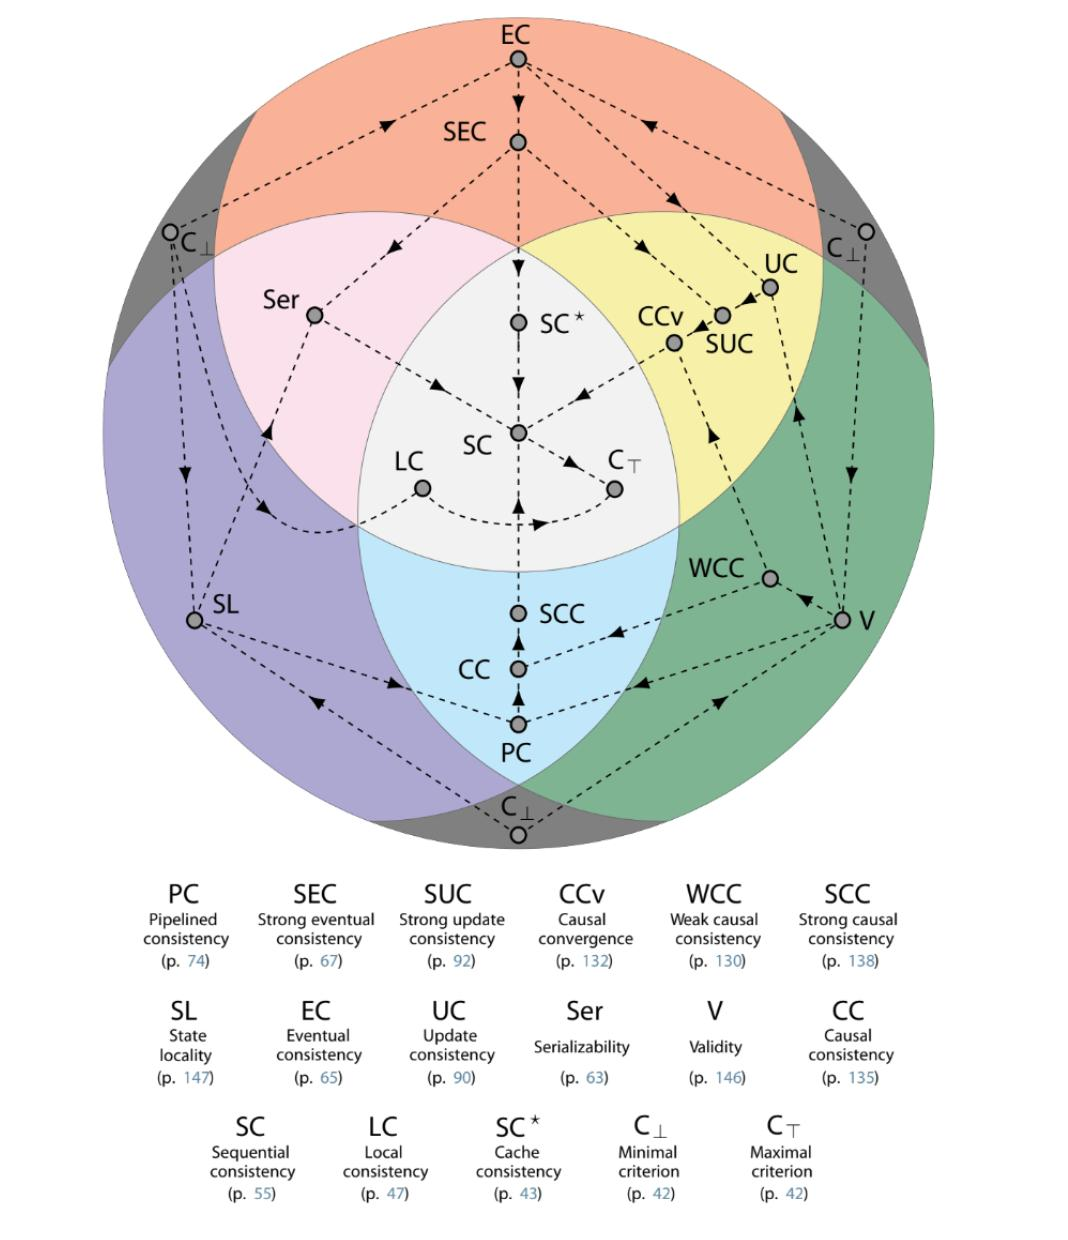
\includegraphics[width=1.1\linewidth,keepaspectratio]{images/perrin_consistencies.png}
        \end{center}
        
        \column{0.5\textwidth}
        \begin{enumerate}
            \item \textbf{Strong Consistency} \\
            Все операции читают последнее записанное значение
            
            \item \textbf{Sequential Consistency} \\
            Существует общий линейный порядок операций
            
            \item \textbf{Causal Consistency} \\
            Happens-before порядок сохраняется
            
            \item \textbf{Eventual Consistency} \\
            Спустя какое-то время реплики сойдутся

            \item \textbf{Strong Eventual Consistency} \\
            Реплика = множество полученных ей сообщений
        \end{enumerate}
\end{columns}

\end{frame}

\begin{frame}
\frametitle{Спектр моделей согласованности}

\begin{columns}
\column{0.5\textwidth}
\textbf{Сильные модели}
\begin{itemize}
    \item Strong Consistency
    \item Sequential Consistency
\end{itemize}


\column{0.5\textwidth}
\textbf{Слабые модели}
\begin{itemize}
    \item Eventual Consistency
    \item Strong Eventual Consistency
    \item Causal Consistency
    \item Session Consistency
\end{itemize}

\end{columns}

\end{frame}

\begin{frame}
\frametitle{Strong Consistency}

\begin{center}
    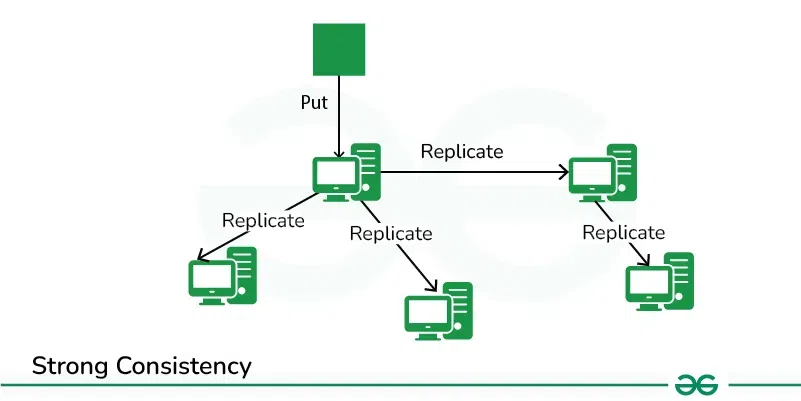
\includegraphics[width=0.8\linewidth,keepaspectratio]{images/geeks-for-geeks-strong-сonsistency.png}
\end{center}


\begin{itemize}
  \item «Одна копия»: Все узлы видят операции в одном глобальном порядке, согласованном с wall-clock временем
  \item $+$ Лучше некуда
  \item $-$ Высокая latency из-за коммуникации (консенсус)
  \item Для денег, персональных данных, критичных бизнес-инвариантов
\end{itemize}

\end{frame}

\begin{frame}
\frametitle{Sequential Consistency}

\begin{itemize}
  \item Схема репликации такая же, как и со strong consistency, но:
  \begin{itemize}
    \item Операция считается принятой {\bfseries до} тех пор, пока она будет применена на всех репликах
    \item Но все еще существует единый глобальный порядок всех операций
    \item Порядок не обязан совпадать с wall-clock временем
  \end{itemize}
\end{itemize}

\begin{block}{Следствие}
Операция, завершившаяся раньше по wall-clock, может оказаться позже в глобальном порядке.
\end{block}

\end{frame}

\begin{frame}
\frametitle{Strong vs. Sequential Consistency}

\begin{center}
\begin{tabular}{p{0.5\linewidth}p{0.25\linewidth}p{0.25\linewidth}}
\textbf{Свойство} & \textbf{Strong} & \textbf{Sequential} \\ \hline
Единый порядок операций & Да & Да \\
Учет реального времени & Да & Нет \\
Влияние сетевых задержек & Выше & Ниже \\
\end{tabular}
\end{center}

\vspace{0.2cm}
\textbf{Грубо говоря:} strong = sequential + real-time constraints.

\end{frame}

\begin{frame}
\frametitle{Семейство моделей Weak Consistency}

    \begin{center}
        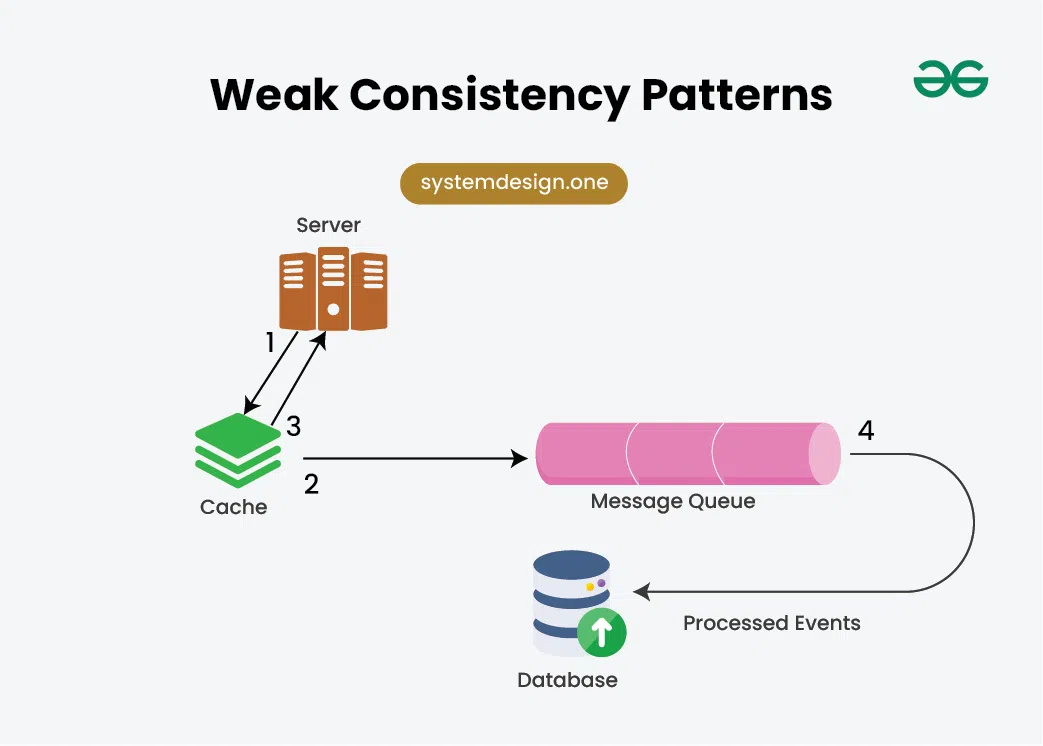
\includegraphics[width=0.6\linewidth,keepaspectratio]{images/geeks-for-geeks-weak-consistency.png}
    \end{center}

\begin{itemize}
  \item Часто дают локальные гарантии:
  \begin{itemize}
    \item Read Your Writes – видим результаты своих же записей
    \item Monotonic Reads – новое чтение не вовращает старые значения
    \item Monotonic Writes – новая запись побеждает старую запись
    \item Writes Follow Reads – если прочитал значение, не перезапишешь его старым
  \end{itemize}
\end{itemize}

\end{frame}

\begin{frame}
\frametitle{Eventual Consistency}

\begin{center}
    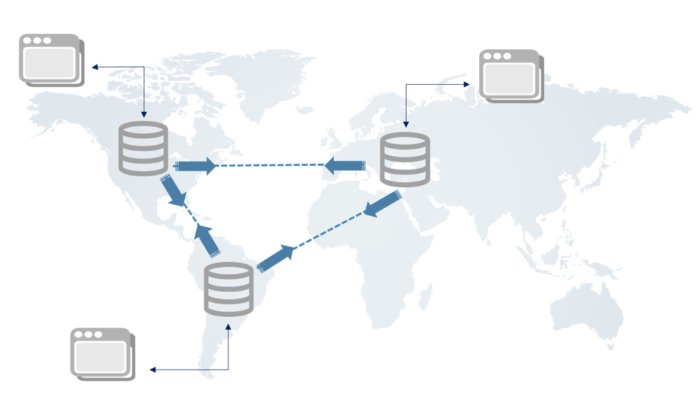
\includegraphics[width=0.5\linewidth,keepaspectratio]{images/redis-crdt-figure-1-100771514-large.jpg}
\end{center}

\begin{itemize}
  \item Если новые записи прекратились, все реплики в итоге сходятся
  \item Не гарантирует срок сходимости
  \item На практике требуется:
  \begin{itemize}
    \item анти-энтропия
    \item детерминированный merge
    \item контроль clock skew (для LWW)
  \end{itemize}
\end{itemize}

\textbf{Типичный сценарий:} кеши, каталоги, ленты рекомендаций.

\end{frame}

\begin{frame}
\frametitle{Causal Consistency}

\begin{itemize}
  \item Сохраняет отношение happens-before между причинно связанными операциями
  \item Конкурентные (независимые) записи могут наблюдаться в разном порядке
  \item Пример:
  \begin{itemize}
    \item пользователь A публикует пост
    \item пользователь B отвечает на пост
    \item нельзя увидеть ответ, не увидев исходный пост
  \end{itemize}
\end{itemize}

\textbf{Механизмы:} vector clocks, dependency tracking.

\end{frame}

\begin{frame}
\frametitle{Strong Eventual Consistency}

\begin{center}
    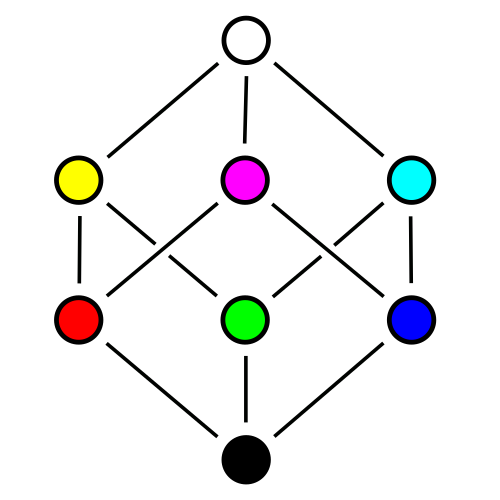
\includegraphics[width=0.2\linewidth,keepaspectratio]{images/crdt-favicon.png}
\end{center}

\begin{itemize}
  \item При доставке одного и того же набора обновлений все реплики гарантированно равны
  \item Порядок доставки не важен
  \item Обычно достигается через CRDT:
  \begin{itemize}
    \item операции коммутативны
    \item merge ассоциативен, коммутативен и идемпотентен
  \end{itemize}
\end{itemize}

\textbf{Примеры:} счетчики, множества, совместное редактирование документов.

\end{frame}

\begin{frame}
\frametitle{Session Consistency}

\begin{center}
    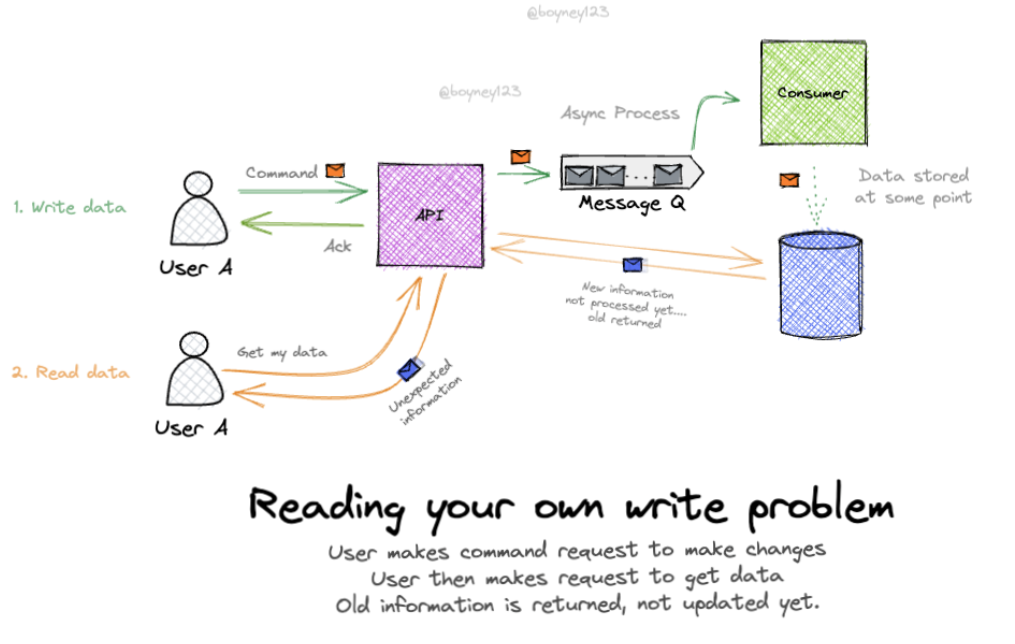
\includegraphics[width=0.8\linewidth,keepaspectratio]{images/read-your-write.png}
\end{center}

\begin{itemize}
  \item Гарантии только внутри одной клиентской сессии (sticky sessions или session token с версией)
\end{itemize}

\end{frame}

\begin{frame}
\frametitle{Как выбирать модель согласованности на практике}

\begin{enumerate}
  \item Выписать бизнес-инварианты (что \textbf{никогда} нельзя нарушить)
  \item Разделить операции на критичные и некритичные
  \item Назначить минимальную достаточную модель на операцию
  \begin{itemize}
    \item платеж/списание: strong или serializable транзакции
    \item лента/счетчики просмотров: eventual или causal
    \item профиль пользователя: session guarantees часто достаточно
  \end{itemize}
  \item Контролировать production через p95/p99 latency и частоту конфликтов
\end{enumerate}

\end{frame}


\section{Сериализуемость транзакций}



\begin{frame}
\frametitle{Что такое серийное расписание?}

\begin{definitionbox}[Серийное расписание]
Серийное расписание — это расписание, в котором транзакции выполняются по одной: 
сначала все операции одной транзакции, затем другой, без чередования.
\end{definitionbox}

% \begin{center}
%     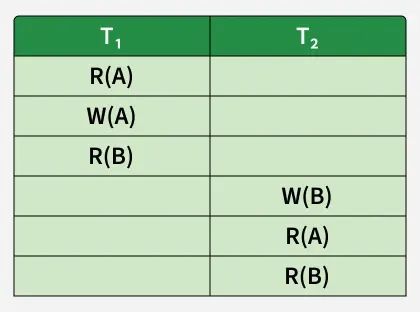
\includegraphics[width=0.6\linewidth,keepaspectratio]{images/gfg-serial-schedule.png}
% \end{center}

% https://www.includehelp.com/dbms/classification-of-schedules-in-dbms.aspx

\begin{center}
    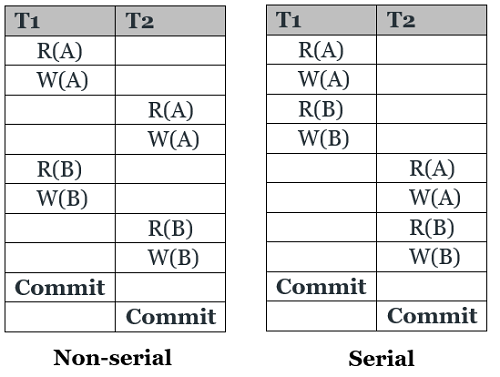
\includegraphics[width=0.6\linewidth,keepaspectratio]{images/serial-schedule.png}
\end{center}

\end{frame}

\begin{frame}
\frametitle{Что такое сериализуемое расписание?}

\begin{definitionbox}[Сериализуемое расписание]
Расписание называется сериализуемым, если оно эквивалентно некоторому серийному расписанию.
\end{definitionbox}

\begin{columns}
\column{0.5\textwidth}
\begin{center}
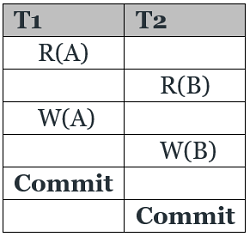
\includegraphics[width=0.6\linewidth,keepaspectratio]{images/types-of-schedules-2.jpg}

Несерийное расписание
\end{center}

\column{0.5\textwidth}
\begin{center}
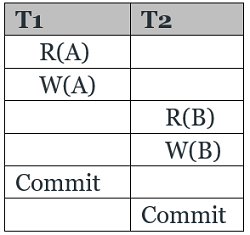
\includegraphics[width=0.6\linewidth,keepaspectratio]{images/types-of-schedules-3.jpg}

Серийное расписание
\end{center}

\end{columns}

\vspace{0.3cm}
Оба расписания выше эквивалентны друг другу. Они сериализуемые.


\end{frame}
% \begin{frame}
% \frametitle{Конфликтно-сериализуемость}



% \end{frame}

\begin{frame}{Конфликтно-сериализуемость}

\begin{definitionbox}
Расписание называется конфликтно-сериализуемым, если его можно превратить 
в серийное, переставляя только неконфликтующие операции.
\end{definitionbox}

\textbf{Две операции конфликтуют, если:}
\begin{itemize}
    \item они из разных транзакций
    \item работают с одним и тем же объектом
    \item хотя бы одна из них — запись (write)
\end{itemize}

\vspace{0.5cm}

\begin{columns}
\column{0.5\textwidth}
\textit{Конфликт:}
\begin{itemize}
    \item $T_1$: write(A)
    \item $T_2$: read(A)
\end{itemize}

\column{0.5\textwidth}
\textit{Нет конфликта:}
\begin{itemize}
    \item $T_1$: read(A)
    \item $T_2$: read(A)
\end{itemize}
\end{columns}

\end{frame}


\begin{frame}{Конфликтно-сериализуемость}

\begin{center}
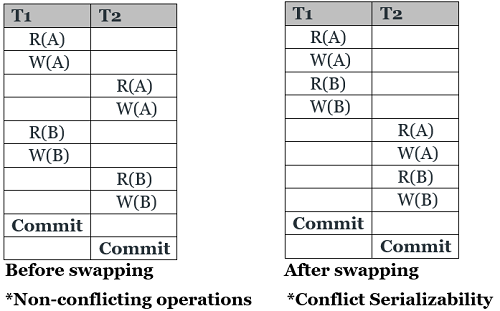
\includegraphics[width=1.0\linewidth,keepaspectratio]{images/types-of-schedules-4.jpg}
\end{center}

\end{frame}

\begin{frame}[fragile]
\frametitle{Разбор задачи: формулировка}

\small
Даны две транзакции:

\begin{verbatim}
T1:
  a = A.getBalance();
  A.credit(INTEREST * a);

T2:
  A.debit(100);
  B.credit(100);
\end{verbatim}

\normalsize
\begin{itemize}
  \item Предположение: каждая операция на объекте атомарна
  \item Нужно: перечислить все interleavings и для каждого ответить:
  \begin{itemize}
    \item это serial execution?
    \item это conflict-serializable execution?
  \end{itemize}
\end{itemize}

\end{frame}

\begin{frame}
\frametitle{Interleaving \#1}

\vspace{0.5em}
\normalsize
\begin{center}
\begin{tabular}{c|p{0.42\textwidth}|p{0.42\textwidth}}
\textbf{Шаг} & \textbf{$T_1$} & \textbf{$T_2$} \\ \hline
1 & \texttt{A.getBalance()} &  \\
2 & \texttt{A.credit(INTEREST * a)} &  \\
3 &  & \texttt{A.debit(100)} \\
4 &  & \texttt{B.credit(100)} \\
\end{tabular}
\end{center}

\vspace{0.4em}
\pause
\textbf{Serial:} да ($T_1 \rightarrow T_2$). \quad
\pause
\textbf{Conflict-serializable:} да.

\end{frame}

\begin{frame}
\frametitle{Interleaving \#2}

\vspace{0.5em}
\normalsize
\begin{center}
\begin{tabular}{c|p{0.42\textwidth}|p{0.42\textwidth}}
\textbf{Шаг} & \textbf{$T_1$} & \textbf{$T_2$} \\ \hline
1 & \texttt{A.getBalance()} &  \\
2 &  & \texttt{A.debit(100)} \\
3 & \texttt{A.credit(INTEREST * a)} &  \\
4 &  & \texttt{B.credit(100)} \\
\end{tabular}
\end{center}

\vspace{0.4em}
\pause
\textbf{Serial:} нет. \quad
\pause
\textbf{Conflict-serializable:} нет (цикл $T_1 \leftrightarrow T_2$).

\end{frame}

\begin{frame}
\frametitle{Interleaving \#3}

\vspace{0.5em}
\normalsize
\begin{center}
\begin{tabular}{c|p{0.42\textwidth}|p{0.42\textwidth}}
\textbf{Шаг} & \textbf{$T_1$} & \textbf{$T_2$} \\ \hline
1 & \texttt{A.getBalance()} &  \\
2 &  & \texttt{A.debit(100)} \\
3 &  & \texttt{B.credit(100)} \\
4 & \texttt{A.credit(INTEREST * a)} &  \\
\end{tabular}
\end{center}

\vspace{0.4em}
\pause
\textbf{Serial:} нет. \quad
\pause
\textbf{Conflict-serializable:} нет (цикл $T_1 \leftrightarrow T_2$).

\end{frame}

\begin{frame}
\frametitle{Interleaving \#4}

\vspace{0.5em}
\normalsize
\begin{center}
\begin{tabular}{c|p{0.42\textwidth}|p{0.42\textwidth}}
\textbf{Шаг} & \textbf{$T_1$} & \textbf{$T_2$} \\ \hline
1 &  & \texttt{A.debit(100)} \\
2 & \texttt{A.getBalance()} &  \\
3 & \texttt{A.credit(INTEREST * a)} &  \\
4 &  & \texttt{B.credit(100)} \\
\end{tabular}
\end{center}

\vspace{0.4em}
\pause
\textbf{Serial:} нет. \quad
\pause
\textbf{Conflict-serializable:} да (эквивалент $T_2 \rightarrow T_1$).

\end{frame}

\begin{frame}
\frametitle{Interleaving \#5}

\vspace{0.5em}
\normalsize
\begin{center}
\begin{tabular}{c|p{0.42\textwidth}|p{0.42\textwidth}}
\textbf{Шаг} & \textbf{$T_1$} & \textbf{$T_2$} \\ \hline
1 &  & \texttt{A.debit(100)} \\
2 & \texttt{A.getBalance()} &  \\
3 &  & \texttt{B.credit(100)} \\
4 & \texttt{A.credit(INTEREST * a)} &  \\
\end{tabular}
\end{center}

\vspace{0.4em}
\pause
\textbf{Serial:} нет. \quad
\pause
\textbf{Conflict-serializable:} да (эквивалент $T_2 \rightarrow T_1$).

\end{frame}

\begin{frame}
\frametitle{Interleaving \#6}

\vspace{0.5em}
\normalsize
\begin{center}
\begin{tabular}{c|p{0.42\textwidth}|p{0.42\textwidth}}
\textbf{Шаг} & \textbf{$T_1$} & \textbf{$T_2$} \\ \hline
1 &  & \texttt{A.debit(100)} \\
2 &  & \texttt{B.credit(100)} \\
3 & \texttt{A.getBalance()} &  \\
4 & \texttt{A.credit(INTEREST * a)} &  \\
\end{tabular}
\end{center}

\vspace{0.4em}
\pause
\textbf{Serial:} да ($T_2 \rightarrow T_1$). \quad
\pause
\textbf{Conflict-serializable:} да.

\end{frame}

\begin{frame}
\frametitle{Итоги по задаче}

\begin{center}
\begin{tabular}{c|c|c}
\textbf{\#} & \textbf{Serial} & \textbf{Conflict-serializable} \\ \hline
1 & да  & да  \\
2 & нет & нет \\
3 & нет & нет \\
4 & нет & да  \\
5 & нет & да  \\
6 & да  & да  \\
\end{tabular}
\end{center}

\vspace{0.4em}
\begin{itemize}
  \item Всего interleavings: $6$
  \item Serial executions: \textbf{\#1, \#6} (2 из 6)
  \item Conflict-serializable: \textbf{\#1, \#4, \#5, \#6} (4 из 6)
  \item Не conflict-serializable: \textbf{\#2, \#3}
\end{itemize}

\begin{block}{Как проверять быстро}
Для каждого расписания достаточно выписать конфликтные пары на $A$ и проверить, возник ли цикл между $T_1$ и $T_2$.
\end{block}

\end{frame}






\section{Транзакционность}

\begin{frame}
\frametitle{Транзакционная модель ACID}

\begin{itemize}
  \item \textbf{Atomicity}: транзакция либо целиком применена, либо откат
  \item \textbf{Consistency}: переход между корректными состояниями БД
  \item \textbf{Isolation}: параллельные транзакции не мешают и не заметны друг другу
  \item \textbf{Durability}: после commit данные переживают сбой узла (WAL)
\end{itemize}

\begin{block}{Важно}
ACID --- это свойства \textit{модели выполнения транзакций}, а не «strong consistency». Но сам подход является пессимистическим.
\end{block}

\end{frame}


\begin{frame}
\frametitle{2PC: 2-Phase Commit}

\begin{center}
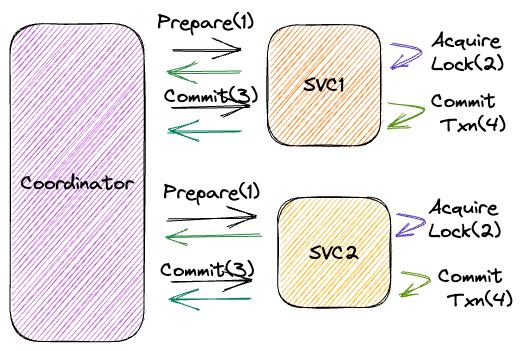
\includegraphics[width=1.0\linewidth,keepaspectratio]{images/2pc.png}
\end{center}

\end{frame}

\begin{frame}
\frametitle{2PL: 2-Phase Locking}

\begin{center}
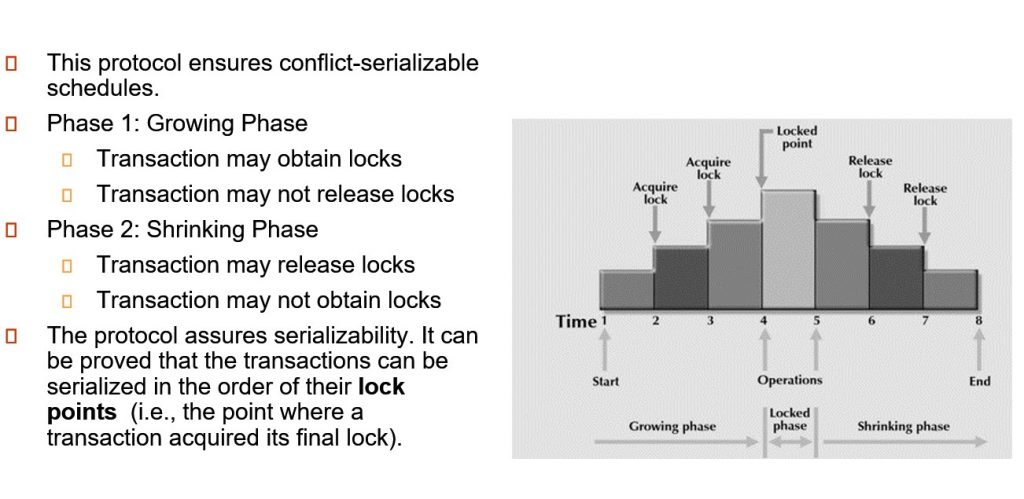
\includegraphics[width=1.0\linewidth,keepaspectratio]{images/2pl-1024x499.jpg}
\end{center}

\end{frame}

%--------------------------------------------------

\begin{frame}{Задача 1: ACID и 2PL}

Если мы просто связываем блокировки (locks) с объектами в транзакционной системе,
чтобы реализовать двухфазную блокировку (2PL),

\begin{itemize}
    \item какие свойства ACID выполняются автоматически,
    \item а какие требуют дополнительной реализации?
\end{itemize}

\vspace{0.5em}

\textbf{Почему?}

\end{frame}


\begin{frame}{Разбор задачи 1}

\pause
\textbf{Atomicity (Атомарность)} — \textbf{требует доп. механизмов}
\small
\begin{itemize}
    \item при сбое изменения могут остаться частично применёнными
    \item нужны undo-логи / rollback
\end{itemize}

\vspace{0.7em}

\pause
\textbf{Consistency (Согласованность)} — \textbf{не гарантируется самим 2PL}
\small
\begin{itemize}
    \item если транзакция сама нарушает инварианты, 2PL это не предотвратит
    \item согласованность обеспечивается корректностью кода и ограничениями БД
\end{itemize}

\vspace{0.7em}

\pause
\textbf{Isolation (Изолированность)} — \textbf{обеспечивается}
\begin{itemize}
    \small
    \item поскольку гарантирует конфликтную сериализуемость
\end{itemize}

\vspace{0.7em}

\pause
\textbf{Durability (Долговечность)} — \textbf{требует доп. механизмов}
\small
\begin{itemize}
    \item 2PL не гарантирует сохранение данных после commit
    \item данные могут быть потеряны при сбое (например, в памяти)
    \item нужны WAL и запись на диск
\end{itemize}

\vspace{0.7em}

\textbf{Итог:} 2PL решает только \textbf{Isolation}; остальные свойства требуют
отдельных механизмов.

\end{frame}

%--------------------------------------------------

\begin{frame}{Задача 2: Durability и Atomicity}

Свойство \textbf{Durability (долговечность)} гарантирует, что если транзакция
объявлена зафиксированной (committed), то её результаты сохранятся даже при сбоях
(например, отключении питания).

\vspace{0.7em}

Однако очевидное решение — просто записывать изменения объектов на диск перед
подтверждением транзакции — может привести к проблемам с \textbf{атомарностью}.

\vspace{0.7em}

\textbf{Вопрос:}  
При каких обстоятельствах это может произойти?

\end{frame}

\begin{frame}{Ответ: Durability vs Atomicity}

\textbf{Проблема:} простая запись данных на диск перед commit

\vspace{0.7em}

\textbf{Когда возникает нарушение атомарности:}
\begin{itemize}
    \item транзакция изменяет несколько объектов
    \item изменения пишутся на диск \textbf{по частям}
    \item происходит сбой (crash, power loss) \textbf{в процессе записи}
\end{itemize}

\vspace{0.7em}

\textbf{Что получаем:}
\begin{itemize}
    \item часть изменений уже записана
    \item часть — нет
\end{itemize}

\vspace{0.5em}

\textbf{Итог:}
\begin{itemize}
    \item транзакция не завершена
    \item но её эффекты частично применены
    \item нарушается \textbf{Atomicity (не "всё или ничего")}
\end{itemize}

\vspace{0.7em}

\textbf{Корень проблемы:} нет механизма отката или восстановления

\end{frame}

\begin{frame}{Write-Ahead Logging (WAL)}

\textbf{Идея:} сначала пишем в лог, потом в данные

\vspace{0.7em}

\textbf{Правила WAL:}
\begin{itemize}
    \item \textbf{1. Log before data}
    \begin{itemize}
        \item изменения сначала записываются в лог
        \item только потом — в базу
    \end{itemize}

    \item \textbf{2. Commit after log flush}
    \begin{itemize}
        \item commit разрешён только после записи лога на диск
    \end{itemize}
\end{itemize}

\vspace{0.7em}

\textbf{Что хранится в логе:}
\begin{itemize}
    \item старое значение (undo)
    \item новое значение (redo)
\end{itemize}

\vspace{0.7em}

\textbf{При сбое:}
\begin{itemize}
    \item незавершённые транзакции → \textbf{UNDO}
    \item завершённые, но не записанные → \textbf{REDO}
\end{itemize}


\end{frame}

%--------------------------------------------------

\begin{frame}{Задача 3: Двухфазная блокировка (2PL)}

\begin{definitionbox}[2PL]
Двухфазная блокировка (2PL) — это один из способов обеспечения изоляции
при параллельном выполнении транзакций над несколькими объектами.

\vspace{0.5em}

Она состоит из двух фаз:
\begin{itemize}
    \item фаза роста (lock expansion)
    \item фаза сжатия (lock contraction)
\end{itemize}
\end{definitionbox}

\vspace{0.7em}

\end{frame}

%--------------------------------------------------

\begin{frame}{Планировщик}

\begin{columns}
\column{0.33\textwidth}
\textbf{$T_1$:}
\begin{itemize}
    \item $x = A.read()$
    \item $B.write(x)$
\end{itemize}

\column{0.33\textwidth}
\textbf{$T_2$:}
\begin{itemize}
    \item $x = B.read()$
    \item $C.write(x)$
\end{itemize}

\column{0.33\textwidth}
\textbf{$T_3$:}
\begin{itemize}
    \item $x = C.read()$
    \item $A.write(x)$
\end{itemize}
\end{columns}

\vspace{0.7em}

Предположим, что планировщик транзакций, стремясь обеспечить справедливость,
использует round-robin планирование по строкам кода.

\begin{center}
\begin{tabular}{c|c|c|c}
\textbf{Время} & \textbf{$T_1$} & \textbf{$T_2$} & \textbf{$T_3$} \\ \hline
1 & $x = A.read()$ &  &  \\
2 &  & $x = B.read()$ &  \\
3 &  &  & $x = C.read()$ \\
4 & $B.write(x)$ &  &  \\
5 &  & $C.write(x)$ &  \\
6 &  &  & $A.write(x)$ \\
\end{tabular}
\end{center}

\vspace{0.5em}

Если транзакция заблокирована (ждёт lock), планировщик пропускает её
и переходит к следующей.

\end{frame}

%--------------------------------------------------

\begin{frame}{Задача 3a}

Если использовать \textbf{наивную 2PL} для транзакций $T_1$, $T_2$, $T_3$:

\vspace{0.5em}

\textbf{Вопрос:}  
Какое расписание будет получено?

\end{frame}

\begin{frame}{Решение задачи 3a}

\small
\begin{center}
\begin{tabular}{c|c|c|c}
\textbf{Время} & \textbf{$T_1$} & \textbf{$T_2$} & \textbf{$T_3$} \\ \hline
1 & lock(A), read(A) &  &  \\
2 &  & lock(B), read(B) &  \\
3 &  &  & lock(C), read(C) \\
4 & lock(B), blocked &  &  \\
5 &  & lock(C), blocked &  \\
6 &  &  & lock(A), blocked \\
\end{tabular}
\end{center}

\vspace{0.5em}

\textbf{Результат:} циклическая ждёт-граф: $T_1 \to T_2 \to T_3 \to T_1$.

\vspace{0.3em}

\textbf{Вывод:} наивная 2PL приводит к \textbf{deadlock}.

\end{frame}

%--------------------------------------------------

\begin{frame}{Задача 3b}

Взаимная блокировка (deadlock) — серьёзная проблема для 2PL.

\vspace{0.5em}

Предположим, что система реализует простой детектор дедлоков:
если есть активные транзакции,
но ни одна не может быть выполнена,
тогда все активные транзакции прерываются (abort),
их блокировки освобождаются,
и они перезапускаются в следующей итерации

\vspace{0.5em}

\textbf{Вопрос:}  
Какое расписание возникнет в этом случае?

\end{frame}

\begin{frame}{Решение задачи 3b}

\small
\begin{center}
\begin{tabular}{c|c|c|c}
\textbf{Время} & \textbf{$T_1$} & \textbf{$T_2$} & \textbf{$T_3$} \\ \hline
1 & lock(A), read(A) &  &  \\
2 &  & lock(B), read(B) &  \\
3 &  &  & lock(C), read(C) \\
4 & lock(B), blocked &  &  \\
5 &  & lock(C), blocked &  \\
6 &  &  & lock(A), blocked \\
7 & abort, все &  &  \\
    & откатываются &  &  \\
8 & lock(A), read(A) &  &  \\
9 &  & lock(B), read(B) &  \\
10 &  &  & lock(C), read(C) \\
11 & lock(B), blocked &  &  \\
12 &  & lock(C), blocked &  \\
13 &  &  & lock(A), blocked \\
\end{tabular}
\end{center}

\vspace{0.5em}

\textbf{Проблема:} система входит в \textbf{бесконечный цикл}.

\vspace{0.3em}

\textbf{Вывод:} простое обнаружение дедлока + перезапуск приводит к \textbf{livelock}.

\end{frame}
%--------------------------------------------------

\begin{frame}{Задача 3c}

Livelock также может возникать при наивном разрешении дедлоков.

\vspace{0.7em}

\textbf{Вопрос:}  
Как можно изменить схему из пункта (b), чтобы гарантировать прогресс,
если дедлок обнаружен?

\end{frame}

\begin{frame}{Решение задачи 3c: Приоритеты}

\textbf{Идея:} использовать \textbf{приоритеты} или \textbf{временные метки} для упорядочения транзакций.

\vspace{0.5em}

Это предотвращает livelock, обеспечивая \textbf{детерминированный} порядок разрешения конфликтов.

\vspace{0.5em}

Рассмотрим две основные схемы:

\begin{enumerate}
    \item \textbf{Wait-Die}: старая транзакция ждёт молодую, молодая откатывается
    \item \textbf{Wound-Wait}: старая откатывает молодую, молодая ждёт старую
\end{enumerate}

\end{frame}

%--------------------------------------------------

\begin{frame}{Решение 3c: Wait-Die схема}

\textbf{Правило:} если $T_i$ (старше) конфликтует на lock с $T_j$ (моложе):
\begin{itemize}
    \item $T_i$ ждёт
    \item $T_j$ откатывается (dies)
\end{itemize}

\vspace{0.5em}

\small
\begin{center}
\begin{tabular}{c|c|c|c}
\textbf{Время} & \textbf{$T_1$} & \textbf{$T_2$} & \textbf{$T_3$} \\ \hline
1 & lock(A), read(A) &  &  \\
2 &  & lock(B), read(B) &  \\
3 &  &  & lock(C), read(C) \\
4 & lock(B), ждёт &  &  \\
5 &  & lock(C), ждёт &  \\
6 &  &  & lock(A), dies! \\
7 &  &  & (перезапуск) \\
8 &  & write(C) \checkmark &  \\
9 &  & (завершено) &  \\
10 & write(B) \checkmark &  &  \\
11 & (завершено) &  &  \\
\end{tabular}
\end{center}

\vspace{0.3em}

\textbf{Результат:} гарантирован прогресс! Нет livelock.

\end{frame}

%--------------------------------------------------

\begin{frame}{Решение 3c: Wound-Wait схема}

\textbf{Правило:} если $T_i$ (старше) конфликтует на lock с $T_j$ (моложе):
\begin{itemize}
    \item $T_i$ прерывает (wounds) $T_j$
    \item $T_j$ откатывается
    \item $T_i$ получает lock
\end{itemize}

\vspace{0.5em}

\small
\begin{center}
\begin{tabular}{c|c|c|c}
\textbf{Время} & \textbf{$T_1$} & \textbf{$T_2$} & \textbf{$T_3$} \\ \hline
1 & lock(A), read(A) &  &  \\
2 &  & lock(B), read(B) &  \\
3 &  &  & lock(C), read(C) \\
4 & lock(B), wounds $T_2$ &  &  \\
5 &  & (dies) &  \\
6 &  & (перезапуск) &  \\
7 &  &  & lock(A), wounds $T_3$ \\
8 &  &  & (dies) \\
9 &  &  & (перезапуск) \\
10 & write(B) \checkmark &  &  \\
11 & (завершено) &  &  \\
\end{tabular}
\end{center}

\vspace{0.3em}

\textbf{Результат:} также гарантирован прогресс, старые транзакции приоритизированы.

\end{frame}


\begin{frame}{Задача 3d}

Предположим, что мы знаем, что будем постоянно исполнять транзакции $T_1$, $T_2$, $T_3$
и хотим объединить их в одну, чтобы исключить livelock.

\vspace{0.7em}

\textbf{Вопрос:}  
Как мы можем это сделать, и почему это будет гарантировать отсутствие дедлоков?

\end{frame}

\begin{frame}
\frametitle{Итоги}

\begin{itemize}
  \item (!) Через неделю дедлайн по второму дз
  \item Обсудили модели согласованности, сериализуемость и транзакционность
\end{itemize}

\end{frame}

\end{document}